% !TEX root = ../../numb3rs.tex
\newpage
\subsection{112: Noisy Edge\label{112}}

In this episode an Aerial Anomaly is reported over at least seven locations in Los Angeles. These observations let Charlie plot the aircraft's likely flight path by using a new way of removing noise from noisy signals (``Squish-Squash''). Since this is a sophisticated mathematical method, we first describe a simple analog, the method of least squares. \\

%%%%%%%%%%
\temph{Least Squares}
%%%%%%%%%%

The path of the Aerial Anomaly that Charlie found was curved, but approximating curves well is difficult. There is a general mathematical principle that to understand something complicated it is best to understand a simple case first, so we will discuss how to fit a line through a group of data points in the plane. \\

So now our task is the following. Given some collection of data points in the plane $(x_1,y_1)$, $(x+2,y_2)$, $\cdots$, $(x_n,y_n)$, find the line $y=ax+b$ that ``best'' fits our data. Least Squares defines best as the minimum sum of the squared distance between the line $y=ax+b$ and our data points. \\

	\begin{figure}[H]
	   \centering
	   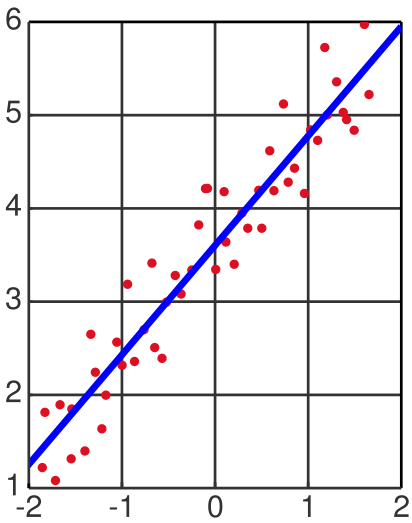
\includegraphics[width=0.3\textwidth]{season1/112/images/data.jpg} 
	\end{figure}

\fbox{\begin{minipage}{43em}
\begin{center} \large \dotuline{Tangent}  \\ \end{center}
Carl Friedrich Gauss developed the fundamentals of Least Squares in 1795 at the age of eighteen. It was used to track the movement of the asteroid Ceres in 1801, based on 40 days of observations, after it was lost in the glare of the sun. For more information click \bref{here}{https://en.wikipedia.org/wiki/Least_squares}.
\end{minipage}} \vspace{0.2cm}

Thus, it is our task to find $a$ and $b$ such that 
	\[
	S= \sum_{i=1}^n (y_i - (ax_i+b))^2
	\]
 is minimized. Now this equation has two parameters that we may vary ($a$ and $b$), so for us to find the minimum we must find where $\frac{\partial S}{\partial a}=0$ and $\frac{\partial S}{\partial b}=0$. (This uses techniques from multivariable calculus. The derivative on the left is a partial derivative with respect to $a$, which means that we treat $a$ as a variable and all the other variables as constants when we take the derivative.) Note, that normally here we would be finding maxima; however this system of equations has only one minimum (since if there were a max we could make it larger by moving $b$ a little further away.) \\

Taking these derivatives, we get
	\[
	\begin{split}
	\frac{\partial S}{\partial a}&= \sum_{i=1}^n -2(y_i-a-bx_i) =0 \\
	\frac{\partial S}{\partial b}&= \sum_{i=1}^n -2x_i(y_i -a-bx_i)=0
	\end{split}
	\]
Rearranging these we get the system of two linear equations with two unknowns. 
	\[
	\begin{split}
	an+b \sum_{i=1}^n \,x_i &= \sum_{i=1}^n \,y_i \\
	a \sum_{i=1}^n \,x_i + b \sum_{i=1}^n \,x_i^2 &= \sum_{i=1}^n \,x_i y_i
	\end{split}
	\]

After inputting the known values for $(x_i, y_i)$ we may then simply solve for the $a$ and $b$ that give us the Least Square Line of our data set.

\fbox{\begin{minipage}{43em}
\begin{center} \large \dotuline{Activity 1}  \\ \end{center}
 Given the data points $(1,5)$, $(2,7)$, $(3,4)$, and $(4,13)$ find, using the last two linear equations, the Least Squares line.
\end{minipage}} \vspace{0.2cm}

\fbox{\begin{minipage}{43em}
\begin{center} \large \dotuline{Activity 2}  \\ \end{center}
Given a set of data points that are co-linear in the plane, show that the Least Squares line is indeed the one that passes through these points.
\end{minipage}} \vspace{0.2cm}

%%%%%%%%%%
\temph{Radars and Signal Processing}
%%%%%%%%%%

In this episode, the stealth capabilities of the Aerial Anomaly make the object unable to be detected by both civilian and military radars. How is it possible that this could happen? Radars work by emitting and receiving electromagnetic radiation. Typically they use the long-wavelength radio and microwaves, because they reflect off of typical aircraft better and are less likely than shorter-wavelength to scatter or be absorbed before returning. Air traffic control radars rotate on a tower emitting \emph{signals} in every direction at the speed of light. When these signals come into contact with objects they are reflected back at the same speed. Measuring the time that it takes for the signal to return lets us calculate the distance to the object. Also, it is known at what angle this signal was emitted, so we know the approximate location of the object. \\

	\begin{figure}[H]
	   \centering
	   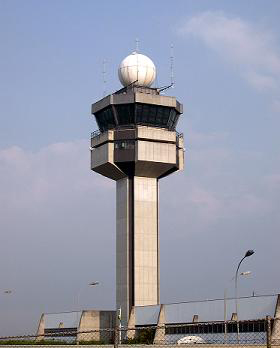
\includegraphics[width=0.3\textwidth]{season1/112/images/tower.jpg} 
	\end{figure}

Its velocity may also be estimated by shifts in the frequency of the signal. If the echo is of a higher frequency it means that object is traveling towards the radar, and lower frequency implies the direction of travel is away from the radar. The magnitude of the change in frequency indicates the speed of the object. \\

	\begin{figure}[H]
	   \centering
	   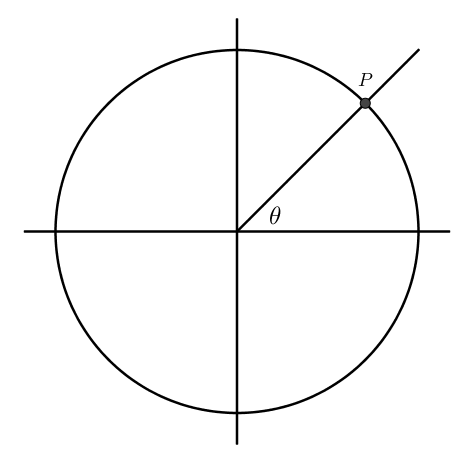
\includegraphics[width=0.5\textwidth]{season1/112/images/circle.png} 
	\end{figure}

However, it is not as ``easy'' as that, the problem is \emph{noise}, which is the mathematical term for errors in measurements. These can be caused by nearby objects, irregularities in the object, or stray radiation. An everyday example of noise is the static on empty TV stations. When trying to find objects such as large jet liners, the reflected \emph{blip} is so strong that the noise is generally insignificant. Airplanes with stealth capabilities reflect so little of the signal that it's hard to tell the difference between their echo and the noise. One nice thing about noise is that it's generally high frequency and the echoes are low frequency. This is also true for the static on tv stations: if you look at any particular pixel in static it will change very frequently, but if you look at a pixel on a tv show, then it will change much less frequently. \\

	\begin{figure}[H]
	   \centering
	   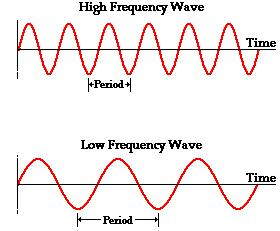
\includegraphics[width=0.5\textwidth]{season1/112/images/hilow.jpg} 
	\end{figure}

Summing these two waves gives us some idea of what the radar would receive when it found an object. To try to remove the noise, one can use an electronic ``low pass filter'' (see \bref{here}{https://en.wikipedia.org/wiki/Low-pass_filter} for more information). If the signals are being processed digitally, then using real-time Fourier Analysis (see \bref{here}{https://en.wikipedia.org/wiki/Fourier_analysis}) can help remove the noise. \\

In this episode, Charlie compares this situation with an audience clapping. Suppose everyone is clapping at a high frequency, except for one person who is clapping at a lower frequency. The single person's clapping sound would be similar to the bottom wave and the rest of the audience's sound would look like the top wave. Recording equipment would record all of these signals at the same time and we could use either type of filter to find the single clapper's frequency. Also, if the slower clapper is clapping with the same loudness and we had 3 recordings, using the idea of the radar in finding distance, we could find (approximately) their location in the room. However, this is not exact, since it is possible for patterns of high frequency waves to look like low frequency waves. This effect is called aliasing (see \bref{here}{https://en.wikipedia.org/wiki/Aliasing} for more information). An example of aliasing called the ``wagon wheel effect'' is visible in most movies that we see. Video equipment is not continuously recording the movements of a car wheel, but rather taking a sampling of images (at say 30~frames/second). Aliasing makes it seem like the wheel is moving more slowly than it actually is, and can even make it look like it is going backwards. \\

Another problem with finding signals of planes with stealth capacity is that the signal may be so weak that the filtering throws it out as noise. However, if the plane is moving at a relatively constant speed we can program the detector to look for patterns in the signal, which will be separated by the distance it travels in consecutive sweeps of the radar. It is assumed that noise will not appear in any coherent pattern, so we may test signals for moving patterns. This is where the reference to ``Squish-Squash'' came up in the episode. To test the data for correlation we must construct a function $g$ (based on our estimate of the speed of the plane) that gives the probability that two data points $p$ and $q$ are related, so that $g(p-q)$ is the probability that $p$ and $q$ are the same object. In other words, if the plane starts at the origin, $g(p)$ is the probability that it will be at the point $p$ one unit of time later. In Noisy Edge, there were 7 sightings of the plane, so using the location and times of the sightings we could estimate the Aerial Anomaly's speed (say it was 20~m/s). Just for simplicity, assume that, after we found the object's expected flight path, we also had a radar directly under its predicted flight path, and that the radar does a full rotation/sec. Then the function $g$ that we might want to use would look like this. 

	\begin{figure}[H]
	   \centering
	   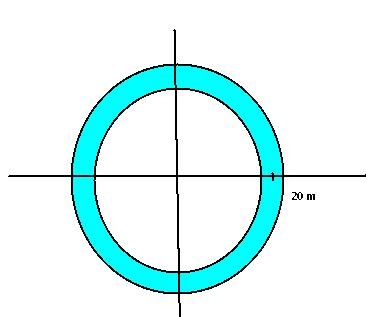
\includegraphics[width=0.5\textwidth]{season1/112/images/squish.jpg} 
	\end{figure}

Here $g$ is 1 in the blue region and 0 outside of the blue region. There are several other more technical things to consider when deciding what the function $g$ should be. After this, if there is a suspected data point we can narrow our search for the plane after one unit of time to the areas for which $g$ has a high value. A recent paper explains how to use this a ``Squish-Squash'' algorithm to modify the function $g$ to make it more likely that data points will be found. It is called ``Continuum Percolation with Unreliable and Spread-Out Connections" by M. Franceschetti et.al., and it appears online \bref{here}{http://circuit.ucsd.edu/~massimo/Journal/JSP-percolation-spread.pdf}. However, this paper requires a significant amount of background to read.

